%==============================================================================
\chapter{Simulation}
\label{sec:sim}
%==============================================================================

As this thesis is about estimating the performance of the PINGU detector before
it is actually built, the estimate has to be based on simulations. In the
chapter on hand, the simulations used to generate the results reported in the
following chapter will be described in detail.

The chapter, as the simulation process, is divided into two sections.
Sec.~\ref{sec:sim_MCchain} will discuss the existing and well-established
IceCube Monte Carlo (MC) chain, which has been adopted for PINGU simulations.
Here, individual neutrino events are generated and their output of Cherenkov
photons is modelled. After propagating the photons through the ice, the
resulting hit pattern is processed through the standard reconstruction and event
selection specified in Secs.~\ref{sec:EvtReco} and \ref{sec:EvtSel},
respectively. The outcome of this event-by-event MC, \ie the effective
areas, reconstruction resolutions, and particle identification efficiencies for
all neutrino flavours, are then used as input for the second part of the
detector simulation.

The Parametric PINGU Analysis, \papa in short, was written specifically for the
rapid analysis of PINGU's neutrino mass hierarchy sensitivity including a
variety of systematic parameters. Since propagating these through the full
MC chain would be way too time-consuming, an effective detector
simulation was implemented that, instead of operating on individual events,
generates the expected event distributions directly, based on the detector
performance retrieved from the MC data. \papa will be described in
detail in Sec.~\ref{sec:papa}.

%==============================================================================
\section{The IceCube/PINGU Simulation Chain}
\label{sec:sim_MCchain}
%==============================================================================

\subsection{Event Generation}
\label{sec:MC_genie}

The first step in the MC chain is to model the interaction of an incoming
neutrino with a target nucleus and the resulting final state, the so-called
event generation. In the dedicated PINGU MC, this is carried out using the
GENIE (Generates Events for Neutrino Interaction Experiments) \cite{GENIE}
software package. This is already the first modification of the standard
IceCube MC chain, where NuGen \cite{NuGen}, an IceCube-specific neutrino
generator, is the default. Yet NuGen is laid out for high-energy neutrino
events where only deep inelastic scattering has to be considered as an
interaction process. In PINGU, however, the low GeV energy range is carrying the
interesting oscillation signal, and here the complex interplay between
quasi-elastic and deep-inelastic scattering as well as resonant processes have
to be taken into account (see Sec.~\ref{sec:XsecsGeV}). Since GENIE puts much
effort into modelling especially this energy range with great care and
validating it against experimental results, it is the natural choice for
generating PINGU events.

GENIE starts off with an isotropic flux of neutrinos of a given flavour
following a user-defined power-law distribution in energy (usually $\propto
E^{-1}$ or $E^{-2}$ for PINGU MC \cite{PINGU_MC}) on the surface of a
cylindrical generation volume well encompassing the full IceCube detector. Any
generated neutrino passing through the interaction volume, which is fully inside
the generation volume but still contains the detector as a whole, is forced to
interact inside this volume. The interaction type is chosen randomly from the
ones that are allowed and the event is assigned a weight $\mathcal{W}_i$
proportional to the particular interaction probability, taking into account the
generated energy spectrum. This weighting strategy makes it possible to
re-weight the generated events to any desired incoming flux $\Phi(E, \theta)$
later on. Then the actual weight is simply given by
\begin{equation}
 w_i = \frac{\Phi(E_i, \theta_i)\,\mathcal{W}_i}{N_\mathrm{evts}} \quad,
 \label{eqn:reweight}
\end{equation}
where $N_\mathrm{evts}$ is the total number of simulated events.

After the interaction mechanism has been determined, the interaction itself is
modelled in detail and all involved particles, from the initial neutrino and
nucleus over possible intermediate states to the final (meta-)stable particles
like pions or muons, are stored inside an \texttt{I3MCTree} object for further
processing. The reference to a tree comes from the fact that this object has
the structure of a multiply nested list, where every particle is the root of a
sub-tree (or branch) holding the particles created in its decay. The particles
are characterised by their identities, positions, four-momenta, and state (such
as 'initial', 'intermediate', or 'final'). 
Additional GENIE-specific information such as the number of generated events,
$N_\mathrm{evts}$, the size of the interaction volume, and others, are kept as
an \texttt{I3MCWeightDict} object.

\subsection{Particle Propagation}
\label{sec:MC_propagation}

The \texttt{I3MCTree} generated by GENIE is handed off to the mmc module
\cite{mmc}, which propagates the final state particles in the tree as well as
possible secondaries created in their decay further through the ice until they
have deposited all their energy. The particles involved here are mainly the
ones involved in the electromagnetic and hadronic showers discussed in
Sec.~\ref{sec:XsecsGeV}, \ie electrons, photons, and pions, respectively, as
well as muons and taus. The \texttt{I3MCTree} is extended with the outcome of
mmc, additional information being stored as \texttt{MMCTrackList} and passed on
to another module called clsim.

clsim \cite{clsim} is then used to generate the Cherenkov photons produced by
the particles propagating through the ice in the detector. Therefore, every
particle is converted into a series of steps of constant velocity $\beta =
v/c$, over which Cherenkov photons are emitted according to
(\ref{eqn:FrankTammWvl}). Usually this process of photon generation is handled
by the Geant4 package \cite{Geant4_1, Geant4_2}, but can also be done using an
effective parametrisation as well.

These photons are then propagated through the ice until they either get absorbed
or hit a DOM. Since photon propagation is a process that can well be run in 
parallel by multiple computation threads, clsim uses the publicly available
OpenCL library \cite{OpenCL} to outsource the calculations to GPUs, resulting
in a significant speedup compared to a simulation on CPUs. The photons that
have collided with a DOM are finally stored in a \texttt{I3MCHitSeriesMap},
containing their parent particle, wavelength, and position and angle of
incidence on the hit DOM. This information gets passed on to emulate the
response of the actual detector.

\subsection{Detector Response}
\label{sec:MC_detector}

In PINGU simulations, all DOMs are represented by an identical copy of the
standard DeepCore DOM, having a 35\,\% higher quantum efficiency than the
IceCube DOMs (see Sec.~\ref{sec:ICDOM}). This is only an approximation of the
actual PINGU DOMs, which currently only exist as prototypes, however it has
already become clear that especially the digitisation process will be
simplified. Yet as the PDOM design is not finalised, the DeepCore DOM is the
closest approximation at hand.

Before the response of the DOMs gets evaluated, noise hits from both thermal
electronic noise as well as radioactive decays inside the DOM and the
accompanying scintillation and fluorescence light are added to the
\texttt{HitSeries} with the vuvuzela module \cite{vuvuzela}. Then the
DOMLauncher module \cite{DOMLauncher} is called to generate the actual DOM
output.

\begin{figure}
\centering
  \subfloat[\label{fig:PMTjitter}]
    {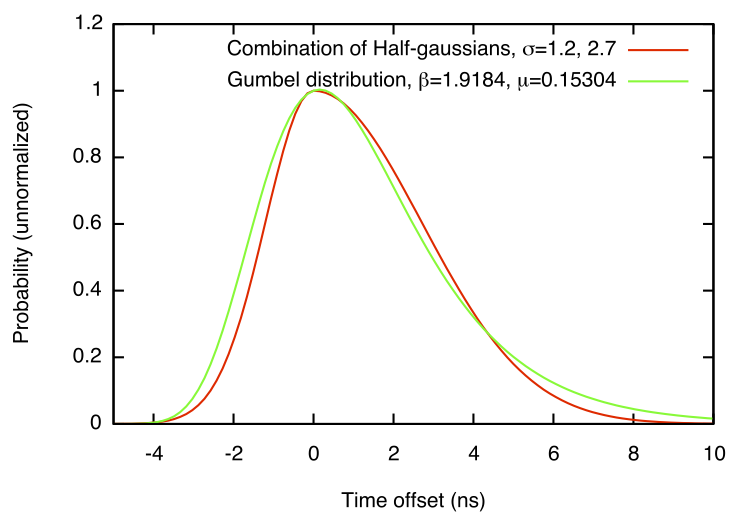
\includegraphics[width=0.5\textwidth]{Jitter_Parameterization}}%\qquad
  \subfloat[\label{fig:SPEcharge}]
    {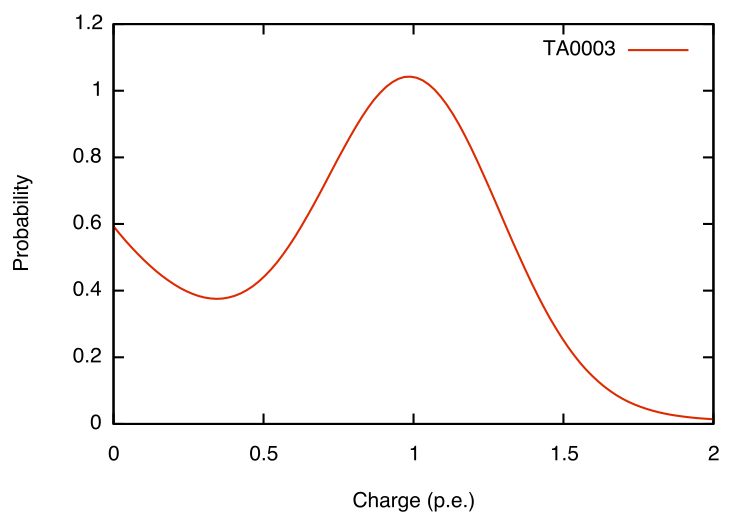
\includegraphics[width=0.5\textwidth]{TA0003}}
  \caption{Parametrisation of \protect\subref{fig:PMTjitter} the PMT transit
       time jitter distribution (in green) and \protect\subref{fig:SPEcharge}
       the single photo-electron charge distribution as used by the
       PMTResponseSimulator. Plots taken from \cite{PMTRes}}
\label{fig:PMTRes}
\end{figure}

The DOMLauncher first calls the PMTResponseSimulator submodule \cite{PMTRes} to
convert the single photo-electron produced at the PMT cathode by a DOM hit to a
charge pulse entering the DOM electronics. Here, the PMT transit time jitter is
applied, meaning that there is a spread in the times needed by the electron
avalanche developing on the PMT dynodes to pass through all amplification
stages. This distribution is shown in Fig.~\ref{fig:PMTjitter}. The
distribution of the amount of charge generated by a single photo-electron is
dominated by a Gaussian, per construction centred at the charge equivalent of
one photo-electron, but also contains a exponentially decreasing component of
small-amplitude pulses, as shown in Fig.~\ref{fig:SPEcharge}.

Once the main photon pulse has been processed, secondary effects like pre-,
late, and afterpulses are added. These result from photons hitting the first
dynode instead of the photocathode, scattered avalanche electrons hitting the
same dynode twice, and ionised residual gas atoms drifting onto the
photocathode, respectively, and are offset by a specific time window from the
main bunch of photo-electrons, but causally connected. Finally, saturation
effects are taken into account, which have to be considered for events of very
high energy or with a vertex in the close proximity of a single DOM.

The full PMT charge output, or waveform, is then passed to the main DOMLauncher
module, which propagates it through the DOM mainboard \cite{DOMLauncher}. First
a discriminator threshold and local coincidence logic are applied, deciding
whether a waveform gets digitised based on its strength and coincidence with a
hit on a neighbouring DOM. These steps will be removed in the actual PDOM since
advances in technology allow a continuous readout of the PMT waveform by a
single ADC instead of the multiple parallel ATWDs \cite{PDOM_Aachen}. Finally,
electronic noise in the digitisers and uncertainties in the time calibration are
added and a digitised representation of the waveform is created, which can then
be injected in the actual reconstruction chain described in
Secs.~\ref{sec:EvtReco} and \ref{sec:EvtSel}.

%==============================================================================
\section{The PaPA Code}
\label{sec:papa}
%==============================================================================

\subsection{Idea}
\label{sec:sim_idea}


\subsection{Implementation}
\label{sec:papa_code}


\subsection{Systematic Parameters}
\label{sec:systematics}
